\section{System Architecture}
\label{sec:sys_arch}

The IOMMU is designed to be flexible and adaptive so that it is possible to integrate it
into various system architecture. The IOMMU works transparently between the peripheral bus
and the memory.

In a transparent configuration, the peripheral bus is not aware of the existence of the
IOMMU. The IOMMU transparently performing address translation for the memory access
requests from the peripheral bus. This configuration is intended for easy integration with
existing systems. This configuration is illustrated by Figure \ref{fig:trans-conf}.

\begin{figure}[ht!]
    \centering
    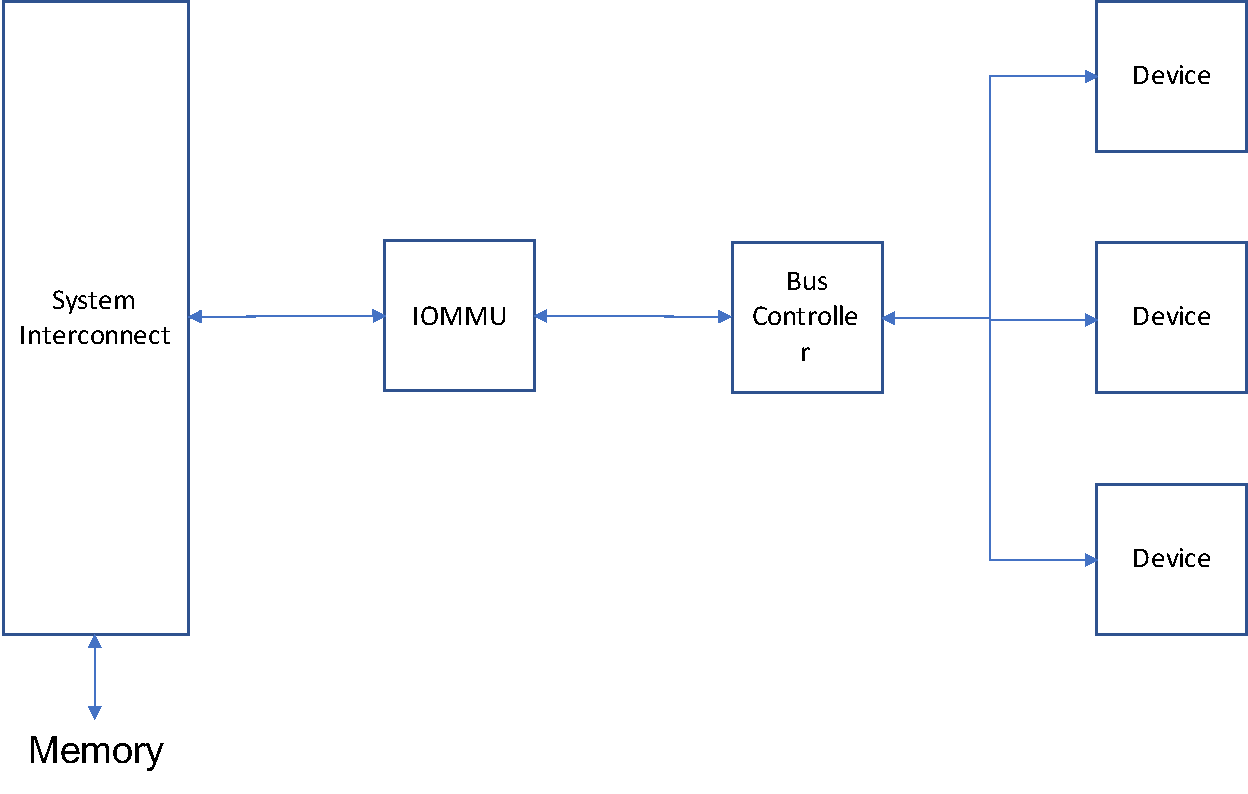
\includegraphics[width=0.95\textwidth]{img/trans-conf.pdf}
    \caption{Transparent Configuration of the IOMMU}
    \label{fig:trans-conf}
\end{figure}

